\chapter{Grundlagen}
TODO

\section{Neuronale Netzwerke}
\subsection{Aktivierungsfunktionen}
\subsection{Fully-Connected Neuronal Network}
\subsection{Convolutional Neuronal Network}
\subsection{Andere Layers}
\subsection{Kostenfunktionen}
\subsection{Backpropagation}
\subsection{Optimierungsalgorithmen}
% Beispiel Abbildung \ref{img:cnn_example_network} mit Zitat.
% \begin{figure}[H]
% 	\centering
% 	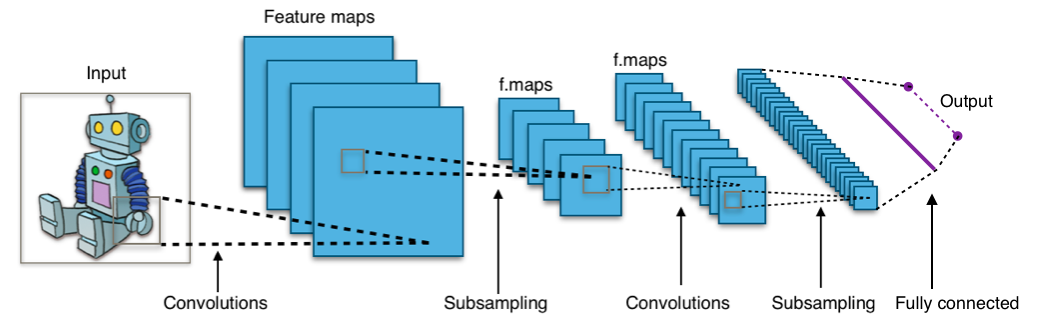
\includegraphics[width=0.95\textwidth]{resources/cnn/typical_cnn}
% 	\caption{Beispiel CNN Arhcitektur \cite{typical_cnn_img}}
% 	\label{img:cnn_example_network}
% \end{figure}

\section{Lab-Farbraum}
\section{Verwandte Arbeiten}
TODO